%% uctest.tex 11/3/94
%% Copyright (C) 1988-2004 Daniel Gildea, BBF, Ethan Munson.
%
% This work may be distributed and/or modified under the
% conditions of the LaTeX Project Public License, either version 1.3
% of this license or (at your option) any later version.
% The latest version of this license is in
%   http://www.latex-project.org/lppl.txt
% and version 1.3 or later is part of all distributions of LaTeX
% version 2003/12/01 or later.
%
% This work has the LPPL maintenance status "maintained".
% 
% The Current Maintainer of this work is Daniel Gildea.

\documentclass[12pt]{ucthesis}
\usepackage{graphicx}
\graphicspath{ {./img} }
\def\dsp{\def\baselinestretch{2.0}\large\normalsize}
\dsp
\begin{document}

% Declarations for Front Matter

\title{Children and IoT Devices}
\author{Yifu Lang}
\degreeyear{2021}
\degreemonth{June}
\degree{MASTER OF SCIENCE}
\chair{Professor Alvaro Cardenas}
\committeememberone{Professor Darrell Long}
\committeemembertwo{Professor David Harrison}
\numberofmembers{3} %% (including chair) possible: 3, 4, 5, 6
\deanlineone{Quentin Williams}
\deanlinetwo{Acting Vice Provost and Dean of Graduate Studies}
\deanlinethree{}
\field{Computer Science and Engineering}
\campus{Santa Cruz}

\begin{frontmatter}

\maketitle
\copyrightpage

\tableofcontents
\listoffigures
\listoftables

% ABSTRACT %%%%%%%%%%%%%%%%%%%%%%%%%%%%%%%%%%%%%%%%%%%%%%%%%%%%%%%%%%%%%%%%%%%%%%%%%%%%
\begin{abstract}
With the recent increase in popularity of the Internet of Things, many companies quickly developed new devices using this technology to stake a claim in a blooming industry. While taking advantage of this technology has yielded many benefits and conveniences in the past few years, the glaring issue of security has not been properly addressed. We have seen many recent attacks on children through IoT devices, and while security mechanisms do exist and are available for use, general users without a technical background may not see the risks as something worth putting effort into mitigating. 

In this thesis, we perform a network analysis on some of the existing products available on the market and collect survey data from parents and their understanding of IoT technologies. We then address the issues in IoT security and provide a solution to persuade more users to be wary of the risks at hand when ignoring proper attention to the protection of their data and privacy. 
\end{abstract}

% DEDICATION %%%%%%%%%%%%%%%%%%%%%%%%%%%%%%%%%%%%%%%%%%%%%%%%%%%%%%%%%%%%%%%%%%%%%%%%%%
\begin{dedication}
\null\vfil
{\large
\begin{center}
To my friends, family,\\\vspace{12pt}
and all who have been there for me through rough times.\\\vspace{12pt}
\end{center}}
\vfil\null
\end{dedication}

% ACKNOWLEDGEMENTS %%%%%%%%%%%%%%%%%%%%%%%%%%%%%%%%%%%%%%%%%%%%%%%%%%%%%%%%%%%%%%%%%%%%
\begin{acknowledgements}
I begin by giving my most sincere gratitude for my thesis advisor, Professor Alvaro Cardenas, as someone who has accompanied me throughout the entire research process and always provided further readings and resources for this thesis.

I would also like to thank Professor Su-hua Wang for guiding me through the process of survey and data collection. Additionally, I extend my gratitude to Elizabeth Goldman, Binaisha Datoor, Adam Ernst, and the entire Baby Lab at UCSC for helping me tread unfamiliar territories in the realm of research.

I want to thank Professor Darrell Long and Professor David Harrison as reading committee chairs for this thesis, and as some of the most influential professors I have had an opportunity to work with in my time at UCSC.

Finally, I want to acknowledge my SASE family, who have inspired me to go above and beyond in my career and have always been a shoulder to lean on when times are tough.

\end{acknowledgements}

\end{frontmatter}

% INTRODUCTION %%%%%%%%%%%%%%%%%%%%%%%%%%%%%%%%%%%%%%%%%%%%%%%%%%%%%%%%%%%%%%%%%%%%%%%%
\chapter{Introduction}
In recent years, society has found an astonishing number of ways to integrate the Internet into day-to-day devices. From smartphones to wearable technology, all devices that are connected to the Internet are encapsulated under the Internet of Things (IoT) \cite{gubbi:iot}. In recent history, modern companies have been finding different ways to incorporate this realm into households; for example, Google and Amazon have extensive development in smart home devices and toy companies have been developing smart toys for children. Overall, the expansion of IoT has enabled massive growth in recent years. Reports have shown that the number of existing Internet-connected devices is projected to grow to 14.7 billion in 2023, 48\% of which accounts for connected home applications, such as smart home devices and security cameras. \cite{cisco}.

However, as a newly blooming technology, the security aspects of these devices are still mostly unexplored. Reports of data leakage and account breaches \cite{wp:camera} for smart devices are rather common as a result of the lack of concern for security on Internet-connected devices; evidently, the importance of implementing security mechanisms into smart devices increases as adversarial parties find new ways to target and attack IoT devices.

Furthermore, with recent expansion of devices for children, parents may be putting their children's at risk. Developers, on the other hand, must also be aware of the additional security measures necessary to satisfy laws such as the Children's Online Privacy Protection Act (COPPA) \cite{reyes:coppa}. As a younger generation becomes more accustommed to an increasingly technological world, we must recognize the risks that children are exposed to when using an IoT device. 

While other works have delved into topics involving smart devices in both security and marketing, we are concerned with a parent's mental model of how IoT and cloud services work and what they are concerned about when their children are exposed to these technologies. We then want to analyze on-the-market products with their cloud architectures and develop a threat model of possible attack vectors. We aim to compare the two models and recommend implementable changes and improvements upon existing features.

In the remainder of this thesis, Chapter \ref{ch:background} begins with exploring the backgrounds of IoT technologies and an analysis of end-user security. Chapter \ref{ch:methodology} explains the methodology of our research process and provides details on our data collection and network analysis. Chapter \ref{ch:mental} and \ref{ch:taxonomy} go into detail on our survey data and technical data, respectively. Finally, chapter \ref{ch:conclusion} concludes our research by recommending security mechanisms to better protect a user's data based on our findings through survey data and network analysis.

% BACKGROUND %%%%%%%%%%%%%%%%%%%%%%%%%%%%%%%%%%%%%%%%%%%%%%%%%%%%%%%%%%%%%%%%%%%%%%%%%%
\chapter{Background}
\label{ch:background}
We begin our investigation by reviewing existing issues found in IoT devices and children's interactions on the Internet.

\section{End-User Perceptions}
While most Internet users understand its inherent risks, it can often be difficult for less experienced users to follow recommended security practices in order to keep their data safe; even the most sophisticated security mechanisms are useless if a user refuses to employ them. Oftentimes, reinforcement learning helps individuals develop habits and pattern recognition, but a lack of concrete results deters these practices. For example, positive outcomes in good cybersecurity awareness include \textit{not} having one's data breached and \textit{not} being the target of an attack. Negative outcomes in bad cybersecurity practices include exposure of data and loss of resources, which may not even occur at all. Research has shown that due to a lack of tangible results in both positive and negative reinforcement in cybersecurity practices, it can often be hard to motivate their integration \cite{west:psychology}.

We aim to model, in general, a parent's perception of modern IoT devices. Previous research conducted by Zeng et al. \cite{zeng:enduser} has shown that smart home users with a technical background tended to better understand cloud infrastructure and how data is collected from a device and transported over a network. Additionally, these users have also shown more concern about the privacy of the data collected by these smart home devices. Inversely, users with less experience with technology tend to show less concern for their data and show little to no understanding of their device's network infrastructure. 

However, a separate study by McReynolds et al. \cite{mcreynolds:toysthatlisten} shows that parents convey more concern for data privacy when their children are involved. When asked questions regarding smart toy and smart device privacy, many parents showed concern for data collection and parental controls, while some of the older children inteviewed expressed concern for a lack of privacy from their own parents.

This investigation may show that parental care plays a role in cybersecurity awareness, which affects a parent's likelihood to purchase and use IoT devices. For our research, our goal is to build a generalizable mental model that encapsulates parents' privacy concerns for their children, understanding of cloud networks, and willingness to allow their children to use a smart device. 

\section{IoT Security Standards}
Smart devices and IoT may open up attack vectors for hackers and other adversaries to take advantage of. Consumers often trust developers and companies to implement sound security mechanisms, or simply are not aware of the importance of their implementation. Unfortunately, there have been many reports of attacks on insufficiently secure devices and applications. For example, an article had found that smart cameras and baby monitors have been at risk due to a lack of security in the mobile applications required to use them. Without mechanisms such as Multi-factored Authentication (MFA), hackers have been able to access the cameras using username-password combinations that were stolen and sold on the Internet \cite{wp:camera}. This process is coined \textit{credential stuffing}.

Dophin attacks, another vector made possible by voice-controlled assistants (VCA), involve ultrasonic sounds inaudible to the human ear that can activate the VCAs built into many IoT devices today \cite{dolphin}. Through dolphin attacks, hackers can sometimes access private data and trigger features unintended by the owner of the device. Attacks like these can often be difficult to predict and prevent due to their invisibility.

Other studies have found hardware issues in devices that could compromise user privacy and data. A study by Streiff et al. \cite{streiff:overpowered} shows that a smart toy by Fischer conceals an Android tablet motherboard. Researchers found that root access to the board was unprotected and that it was easy to gain access to both the camera and microphone built into the toy; it is entirely possible for an attacker to take advantage of this poor design to spy on other consumers.

Evidently, the industry has yet to fully understand each vulnerability that resulted through the widespread usage of IoT technologies. Our research aims to analyze two IoT products and develop a threat model for both, looking for vulnerabilities in their mobile applications, networks, and hardware.

\section{Children's Protection}
Under United States law, children's personal identifiable information is heavily protected under the Children's Online Privacy Protection Act (COPPA). When providing a service or product that is connected to the Internet to children under the age 13, developers are legally required to obtain parental permission and inform users of data collection. Data collection must be kept to a bare minimum for a product to function and collected data must be available for review and deletion.

Ever since COPPA was passed, many tools and resources were created to help developers implement extra measures for protecting children's data. For example, some software development kits (SDK) provide extra options to limit the kinds of data an application is able to collect \cite{reyes:coppa}, and Samet Privacy's kidSAFE\textsuperscript{\textregistered} Seal Program (fig. \ref{fig:kidsafe}) verifies the COPPA-compliance of devices and applications.

While meeting COPPA standards is a legal requirement for any Internet-connected product available in the United States, research has shown that developers often neglect doing so. Reyes et al. \cite{reyes:coppa} have found that out of the top 5,885 children's mobile applications on the Google Play Store analyzed in their study, a majority of them are potentially violating COPPA standards due to misuses of mobile SDKs. This discovery shows that although there are laws in place to ensures the safety of children's data, this industry has yet to fully accomodate for the requirements set through these laws. 

Another study conducted by Le et al. \cite{le:skillbot} delves into the safety of Amazon's VCA Alexa, which found that many children's built-in applications, called \textit{skills}, harbored inappropriate contents and often collected too much data for COPPA-compliance. The study also found that many parents had concerns regarding the content of these skills and often did not take full advantage of parental control features.

\begin{figure}
    \centering
    
\includegraphics[width=0.3\textwidth]{kidsafe1.png}
    
\includegraphics[width=0.3\textwidth]{kidsafe2.png}
    
\includegraphics[width=0.3\textwidth]{kidsafe3.png}
    \caption{The kidSAFE seal of certification helps parents identify Internet-connected products that are verifiably COPPA-compliant.}
    \label{fig:kidsafe}
\end{figure}

With the data and privacy of children at risk, it has become ever so important for developers to be wary of what data their products collect and what content is available to children. Finally, our study aims to find better methods of data collection and suggest implementing several mechanisms that can help ensure children's safety. 

% METHODOLOGY %%%%%%%%%%%%%%%%%%%%%%%%%%%%%%%%%%%%%%%%%%%%%%%%%%%%%%%%%%%%%%%%%%%%%%%%%
\chapter{Methodology}
\label{ch:methodology}
Our research delves into two separate fields. First, we explore end-user psychology through survey data. On the other hand, we also delve into the technical aspects of two existing IoT products that are currently available on the market: Amazon's Echo Dot for Kids is a voice assistant smart home device with parental control and restriction features, and the Roybi Robot is a smart toy designed as a tutor for young children (fig. \ref{fig:devices}).

\begin{figure}
    \centering
    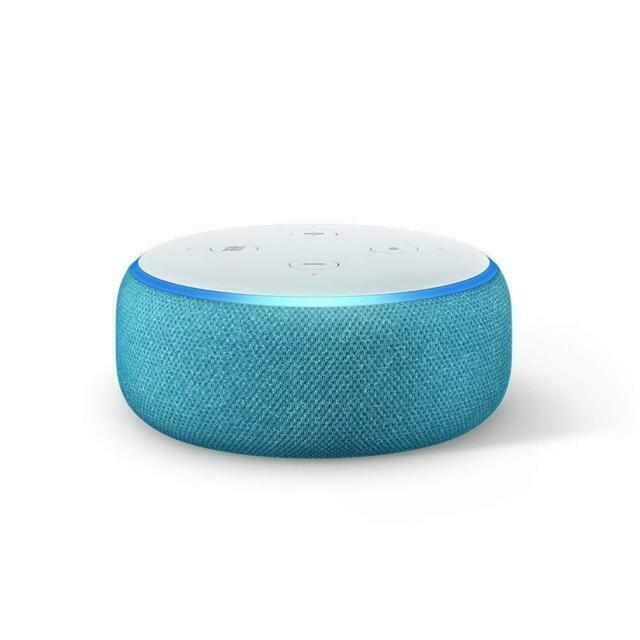
\includegraphics[width=0.3\textwidth]{echo.jpg}
    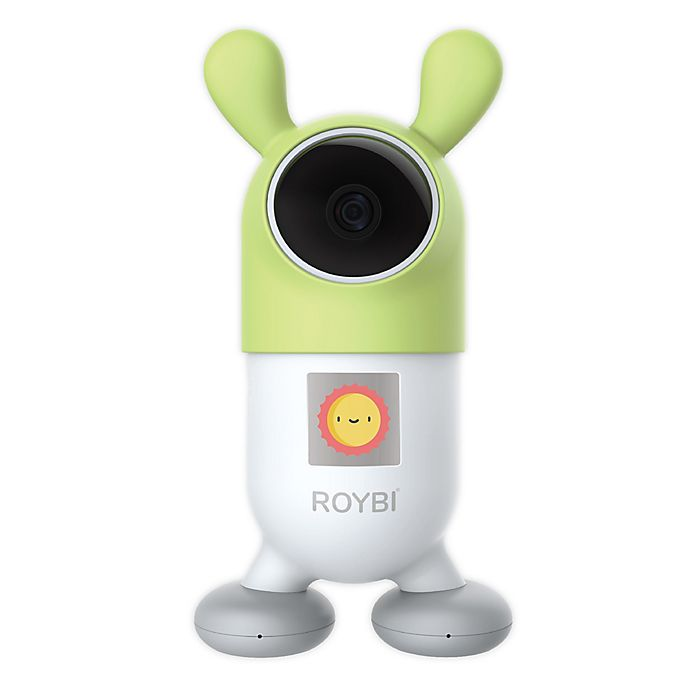
\includegraphics[width=0.3\textwidth]{roybi.jpg}
    \caption{Our research involves analysis of two smart devices designed for children: the Amazon Echo Dot for Kids and the Roybi Robot.}
    \label{fig:devices}
\end{figure}

\section{End-User Mental Model}
We want to understand the psychology involving, parents, IoT, and data privacy through developing a mental model.

\subsection{Privacy Policy}
Both devices presented in the survey have privacy policies to inform users of data collection and what rights the user has. Since devices designed for child use must also comply with COPPA, we can expect to see specific details regarding specific permissions granted by the parents, what data is collected, and how much control parents have over collected data. We review each device's privacy policy and compare our findings from the device taxonomy to reveal any inconsistencies in data collection. We also look into any COPPA violations that could possibly be present in the devices.

\subsection{Survey}
To build a generalizable mental model on parents and IoT devices, we ran a survey (Appendix \ref{app:questions}) to better gauge the experiences and opinions of parents concerning smart devices designed for children. We ask questions regarding their experience with technology, thoughts on smart devices and smart toys, privacy practices, and demographics. Additionally, we show the subjects short videos demonstrating two smart devices designed for children and ask about their thoughts and concerns about them. 

Our survey was conducted through Qualtrics. The research was approved by the University of California, Santa Cruz Institutional Review Board (IRB) and abides by the regulation of the Office of Research Compliance Administration (ORCA). We collected no personal identifiable information except an email, which is deleted from our records as compensation is sent. Our subjects consisted of parents of children ages 6 or younger that are currently residing in the United States. We recruited participants from an existing subject pool from the Baby Lab at UCSC, as well as through word-of-mouth and email. Those who completed the survey were compensated with a \$10 Amazon gift card.

Through the questions asked on the survey, we aim to model several high-level properties of parents and IoT.

\subsubsection{Data Privacy}
As discussed in chapter \ref{ch:background}, previous research has shown that smart device users that are less experienced with technology tend to show less concern for data privacy. We ask questions regarding how our subjects keep their data safe and if they have any concerns regarding data collection in Internet-connected devices. These questions help us understand which data privacy issues parents are aware of, and which issues may require additional scrutiny.

\subsubsection{Cloud Infrastructure}
We want to measure the level of understanding parents have for the cloud infrastructure of the two smart devices we present in the survey. We ask questions gauging the subjects' understanding of how data is collected through the devices, where it is stored, and how it is transferred over a cloud server. 

\subsubsection{Developer Reliability}
We also want to understand the extent to which parents trust the Internet-connected devices that are currently available on the market. We ask for the subject's opinions on the two devices presented in our research, such as what they liked or disliked about the toy and what kind of design improvements could be made. Understanding a parent's trust in children's IoT devices helps us further understand their security weaknesses and shines a light on what features parents are concerned about.

\section{Device Taxonomy}
In the technical aspects of our research, we look into two smart devices designed for children that are available on the market.

\subsection{Network Analysis}
In order to develop threat models for our devices, we investigate the security standards of these devices. Using the Internet Sharing feature on OSX, we used a Macbook as a WiFi endpoint for both devices, as well as a mobile device for the applications used to control them. The laptop connected to a router through an ethernet cable serves as a bridge between the router and our smart devices \ref{fig:experiment}. We then use Wireshark to analyze the network traffic of all of our devices. Details we are looking for include:

\begin{itemize}
    \item Frequency of packets being sent 
    \item Total bandwidth of network traffic 
    \item Servers the devices are in communications with 
    \item Packet protocol
    \item Encryption standards
    \item Possible attack vectors
\end{itemize}

All in all, we are searching for insecure features that may either violate COPPA standards or be an exploitable security flaw.

\begin{figure}
    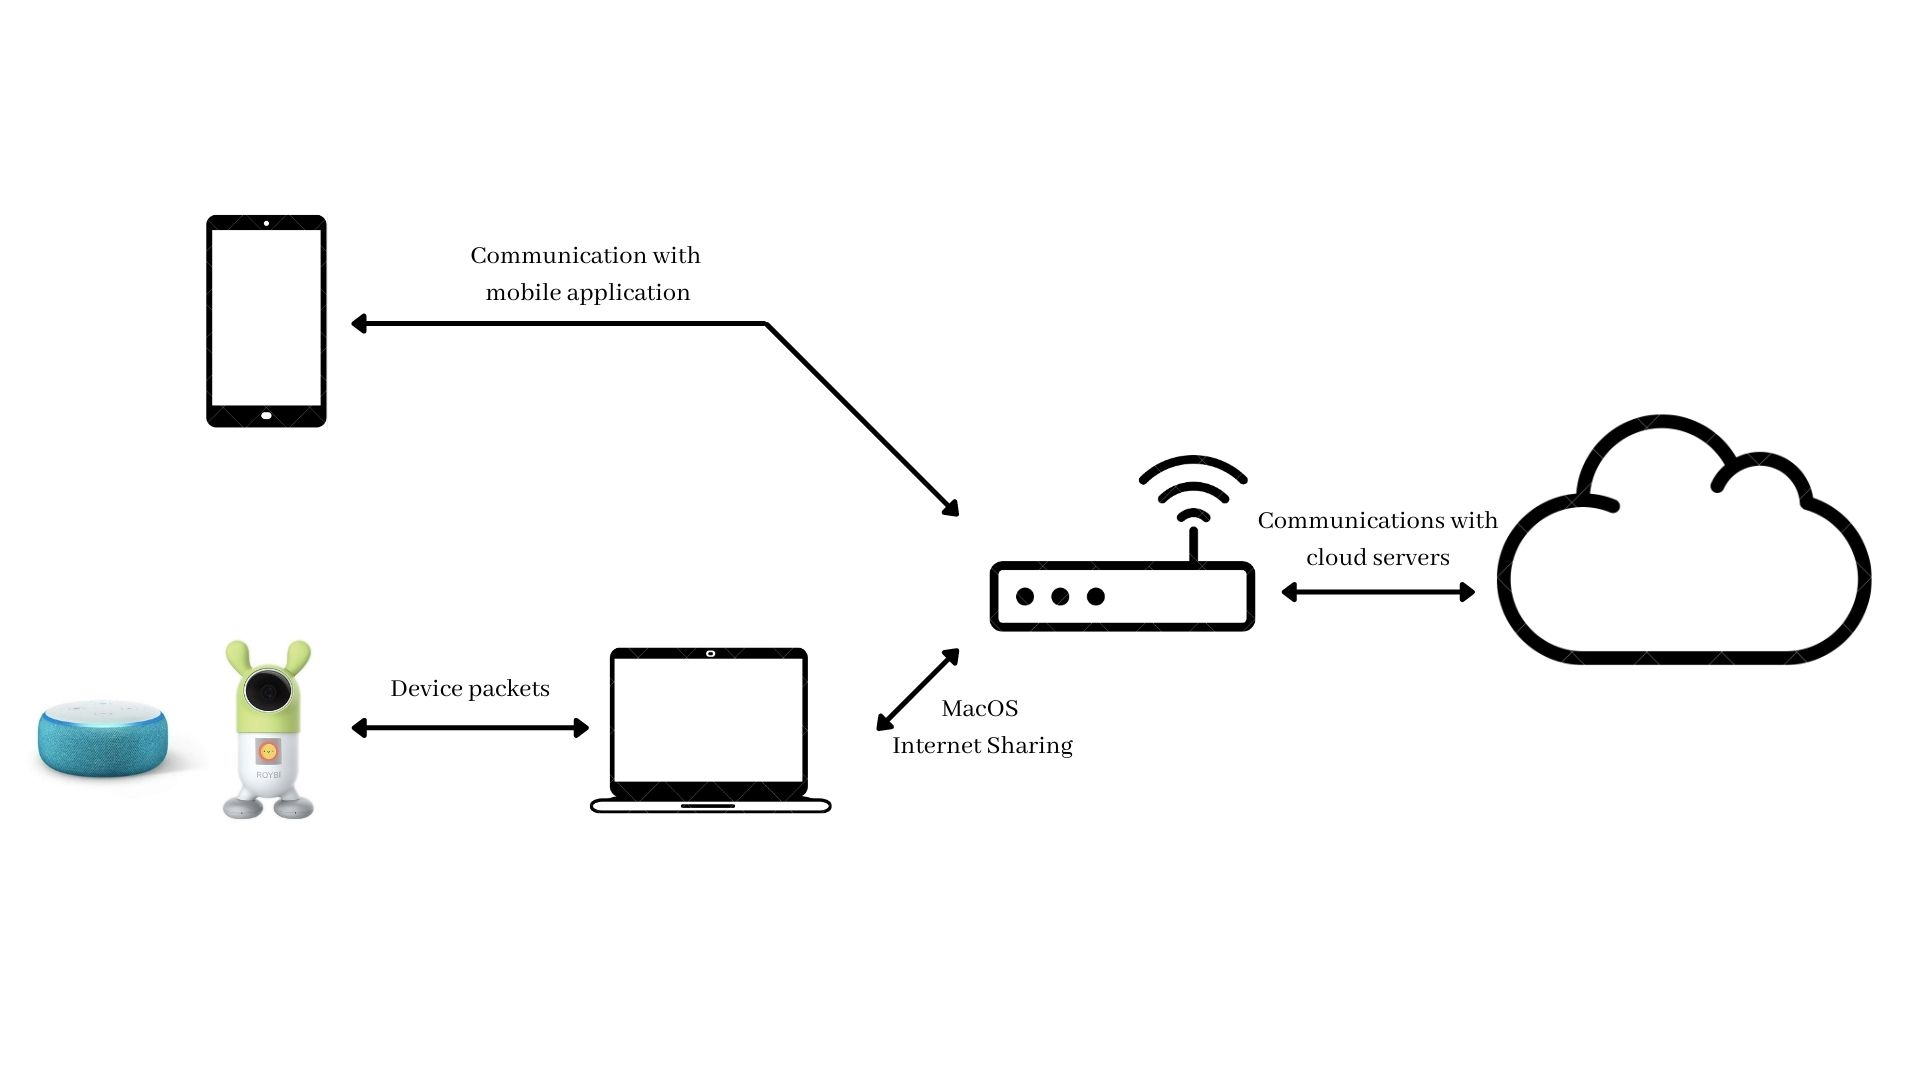
\includegraphics[width=\textwidth]{experiment.jpg}
    \caption{A high level overview of our experiment setup.}
    \label{fig:experiment}
\end{figure}

\subsection{Attack Vectors}
Given the versatility of both the Echo Dot and the Roybi Robot, our research aims to find possible attack vectors for either devices. With the network analysis performed as described in the previous section, we first examine any inconsistencies with encryption protocols and packet patterns to find network exploits. We also examine each feature of both devices to observe any possible COPPA violations or privacy breaches. Finally, we test known attack vectors on the devices. 

The methodology presented in this chapter results in both a mental model of parents and their children's interactions with smart devices and a threat model of the possible attacks or breaches of privacy that could occur in smart device use. We seek to compare these two models in order to recommend changes to be made for a safer IoT environment.

% MENTAL MODEL %%%%%%%%%%%%%%%%%%%%%%%%%%%%%%%%%%%%%%%%%%%%%%%%%%%%%%%%%%%%%%%%%%%%%%%%
\chapter{End User Mental Model}
\label{ch:mental}


% TAXONOMY %%%%%%%%%%%%%%%%%%%%%%%%%%%%%%%%%%%%%%%%%%%%%%%%%%%%%%%%%%%%%%%%%%%%%%%%%%%%
\chapter{Device Taxonomy}
\label{ch:taxonomy}
We perform network analyses on two separate products: Amazon's Echo Dot for Kids and the Roybi Robot, both of which are smart devices designed for children's use. In our analyses, we pay attention to each feature the devices offer and how they communicate with their cloud services and the parent's mobile device through its designated application.

\section{Amazon Echo Dot for Kids}


\section{Roybi Robot}
\begin{figure}
    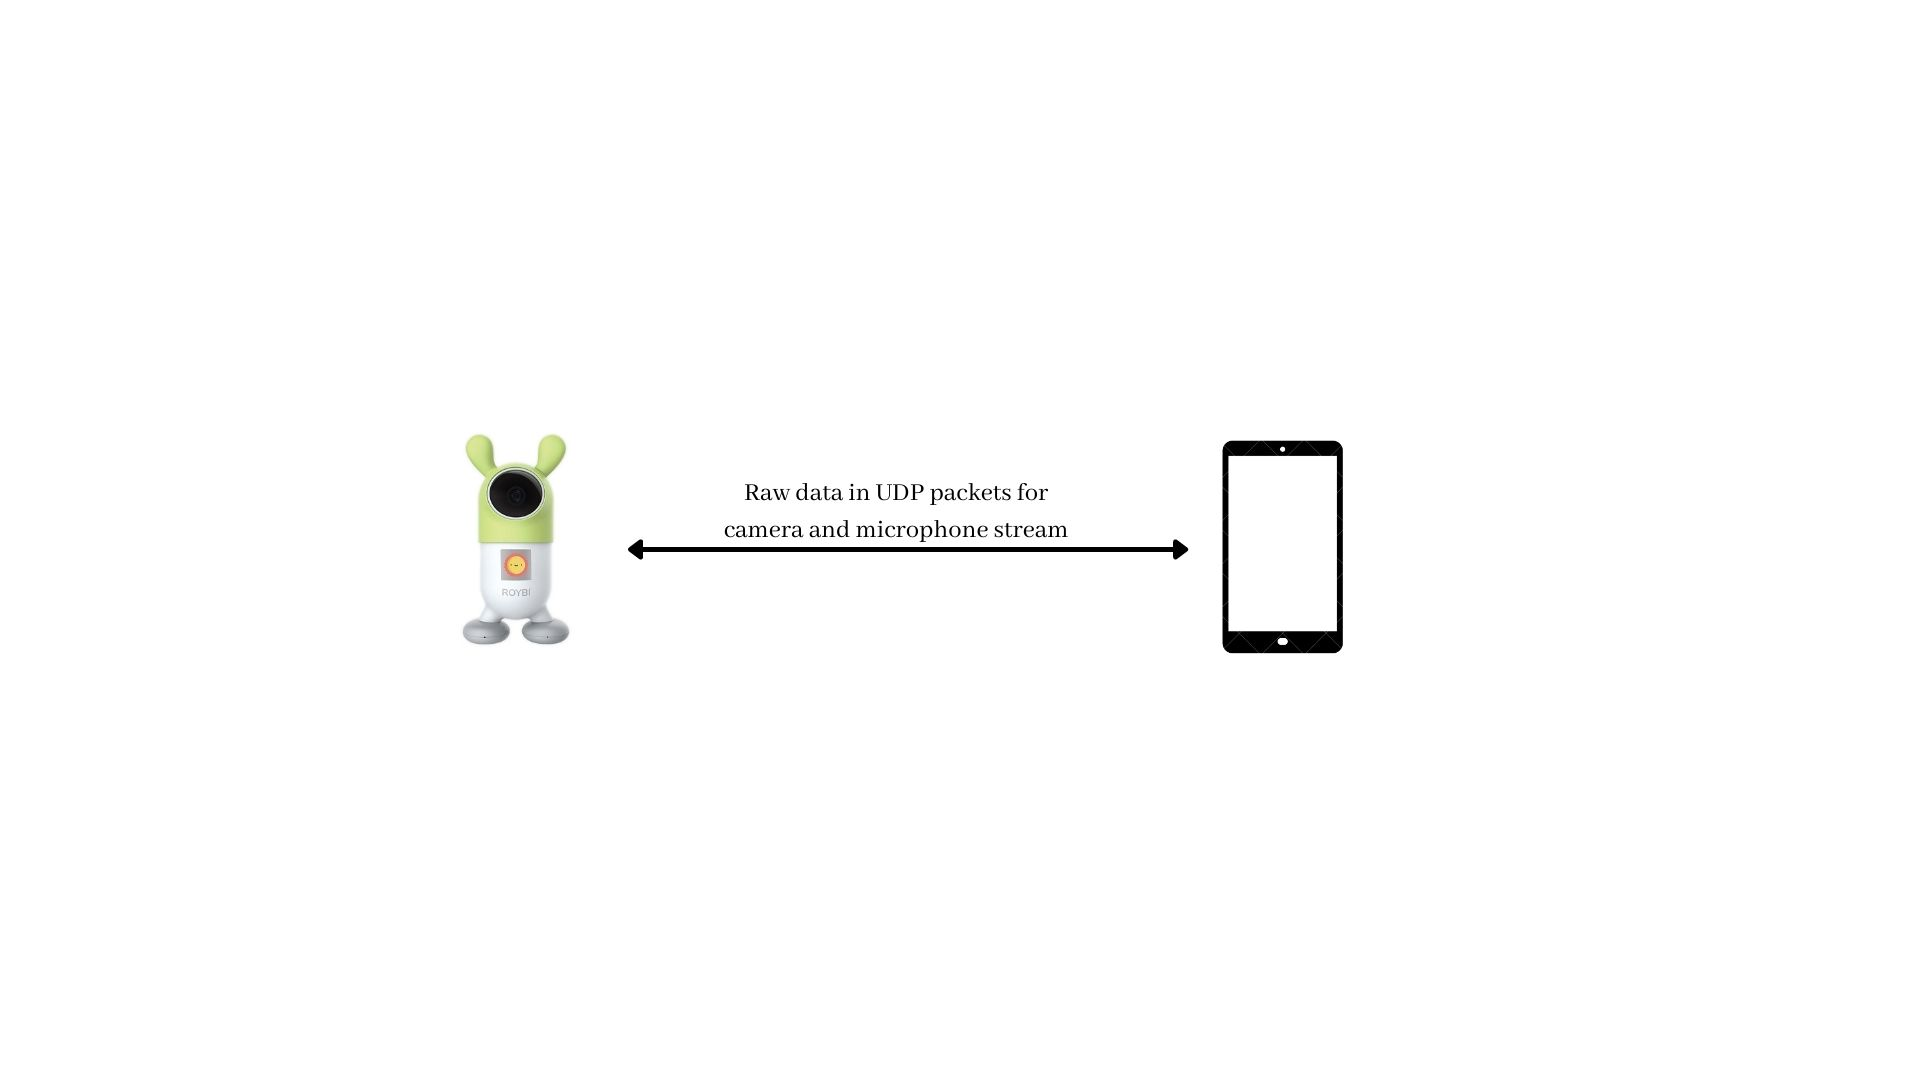
\includegraphics[width=\textwidth]{udp.jpg}
    \caption{Roybi's camera functionality directly connects to the application on the mobile device through a socket. We have found that it contains unencrypted or poorly encrypted data.}
    \label{fig:udp}
\end{figure}

\begin{figure}
    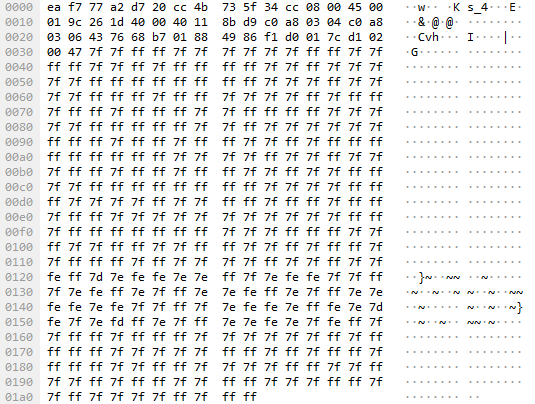
\includegraphics[width=0.5\textwidth]{unencrypted1.png}
    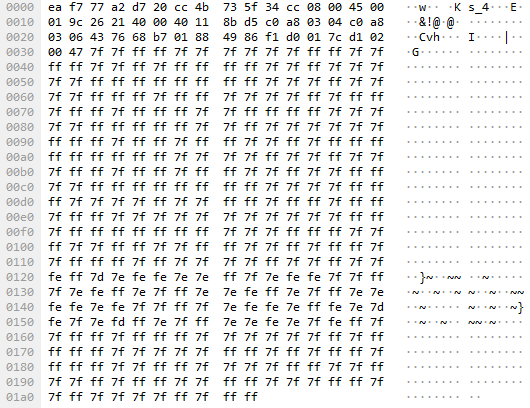
\includegraphics[width=0.5\textwidth]{unencrypted2.png}
    \caption{A Wireshark packet capture shows that the Roybi Robot sends a UDP stream with small differences in data per packet.}
    \label{fig:unencrypted}
\end{figure}

% CONCLUSION %%%%%%%%%%%%%%%%%%%%%%%%%%%%%%%%%%%%%%%%%%%%%%%%%%%%%%%%%%%%%%%%%%%%%%%%%%
\chapter{Conclusion}
\label{ch:conclusion}


% BIBLIOGRAPHY %%%%%%%%%%%%%%%%%%%%%%%%%%%%%%%%%%%%%%%%%%%%%%%%%%%%%%%%%%%%%%%%%%%%%%%%
\nocite{*}
\bibliographystyle{plain}
\bibliography{uctest}


% APPENDIX %%%%%%%%%%%%%%%%%%%%%%%%%%%%%%%%%%%%%%%%%%%%%%%%%%%%%%%%%%%%%%%%%%%%%%%%%%%%
\appendix
\chapter{Survey Questions}
\label{app:questions}
The following section contains the questions we ask in our survey. Some topics include experience with technology, perceptions of our subject devices, data privacy, and demographics.

\begin{itemize}
    \item Smart device related questions
    \begin{itemize}
        \item If you own a smart home device, how long have you been using it?
        \item Does your child have access to a smart home device?
        \item If you own any other smart devices (e.g. smart watch, smart TV, etc.), how long have you been using it?
        \item Does your child use smart devices other than smart home devices?
        \item If you do \textbf{not} own any smart devices, would you consider buying one? Will your child have access to it? Why or why not?
    \end{itemize}
    \item Subject device questions
    \begin{itemize}
        \item Have you heard about this toy/device? If yes, please explain where.
        \item What do you like about the toy/device?
        \item What do you dislike about the toy/device?
        \item Would you consider purchasing the toy/device? If so, why? If not, what kind of improvements would you like to see be made for you to reconsider?
        \item What do you expect to be in the toy/device's privacy policy?
    \end{itemize}
    \item Scale questions (scale on Disagree-Agree)
    \begin{itemize}
        \item I have concerns for how my data is collected and stored on the Internet.
        \item I find it important that collected data is kept private.
        \item I thoroughly research into Internet-connected devices before making a purchase.
        \item I am familiar with the Children’s Online Privacy Protection Act (COPPA).
    \end{itemize}
    \item Data privacy questions
    \begin{itemize}
        \item Please describe your understanding of how Internet-connected devices collect data. 
        \item Please describe your understanding of where and how this data is stored.
        \item Please describe any concerns for how your data is stored on the Internet.
        \item What practices does your family use to keep your data safe?
        \item Have you had any security concerns with devices connected to the Internet?
        \item What concerns do you have about the dialogue between your child and the devices presented in this survey?
    \end{itemize}
    \item Demographics questions
    \begin{itemize}
        \item Age 
        \item Age(s) of children 6 years old or younger
        \item Highest level of education
        \item Occupation
        \item Family household income
        \item Experience with technology
    \end{itemize}
  \end{itemize}
\end{document}
